\documentclass{article}
\usepackage[a4paper, total={6in, 8in}, margin=20mm]{geometry}
\usepackage{graphicx}
\usepackage{hyperref}
\usepackage{sidecap}
\parindent=0pt
\parskip=12pt

\begin{document}
	The OPTIMADE API enables a user to obtain material information from multiple providers with the same filter query. This is particularly useful for machine learning workflows. Being able to query multiple providers using a single API allows a user to combine data from multiple sources, each of which may have different fidelity and focus v. Below, we describe the use of the OPTIMADE API in an exemplar machine learning workflow.
		
	
%	A model trained on data from all the providers (say C) performs quite well when tested on materials from any of the three providers. On the other hand, i
%	
%	When this model is trained on data from all the providers, it performs quite well (R$^2 = 0.98$, see top inset in \autoref{fig: exampleFig}) 
%	
%	
%	than when it is trained on data from only one provider when tested on data from the same pool.  Meanwhile, the model trained on data from call providers (C) retains its predictive power for data from all the providers.
	
	

	\begin{SCfigure}
		\centering
		\caption{asda}
		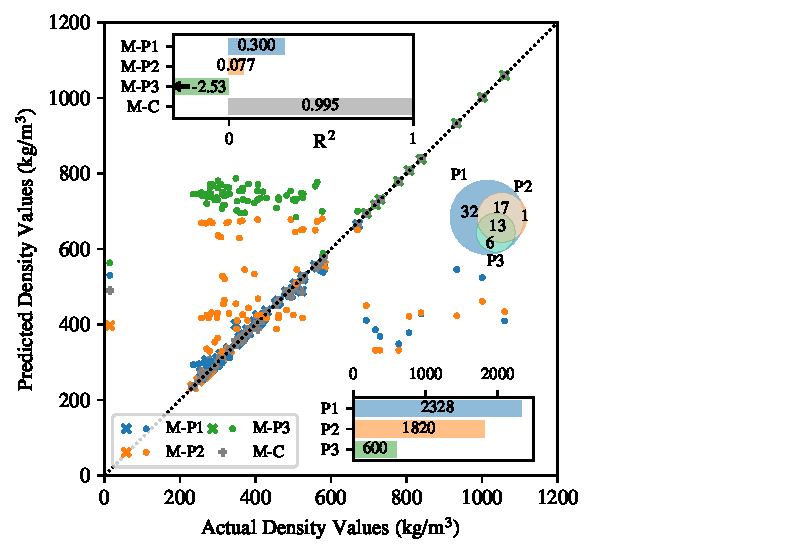
\includegraphics[]{highEntropyExample.pdf}
		\label{fig: }
	\end{SCfigure}
\end{document}